\section{範例與練習}
    \problem 洛谷 P2181

    \textbf{題目敘述}

    對於一個 $n$ 個頂點的凸多邊形,它的任何三條對角線都不會交於一點。求出圖形中對角線交點的個數。

    例如,$6$ 邊形:

    \begin{figure}[!htbp]
        \centering
        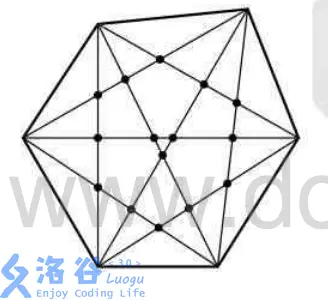
\includegraphics[width=0.5\textwidth]{../Images/Vector2.png}
    \end{figure}

    \textbf{輸入說明}

    輸入只有一行一個整數 $n$,代表邊數。$3 \leq n \leq 10^5$。

    \textbf{輸出說明}

    輸出一行一個整數代表答案。

    \textbf{範例測試}

    \begin{tabular}{|m{7cm}|m{7cm}|}
        \hline
        範例輸入 1 & 範例輸出 1 \\
        \hline
        \verb|4| & \verb|1| \\
        \hline
    \end{tabular}

    \problem 洛谷 P1142 轟炸

    \textbf{題目敘述}

    「我該怎麼辦?」飛行員 klux 向你求助。

    事實上,klux 面對的是一個很簡單的問題,但他實在太菜了。

    klux 要想轟炸某個區域內的一些地方,它們是位於平面上的一些點,但是(顯然地)klux 遇到了抵抗,所以klux 只能飛一次,而且由於飛機比較破,一點起飛就只能沿直線飛行,無法轉彎。現在他想一次轟炸最多的地方。

    \textbf{輸入說明}

    第一行為 $n$

    輸入數據由 $n$ 對整數組成 $(1 \le n \le 700)$,每對整數表示一個點的坐標。沒有一個點會出現兩次。

    \textbf{輸出說明}

    一個整數,表示一條直線能覆蓋的最多的點數。

    \textbf{範例測試}

    \begin{tabular}{|m{7cm}|m{7cm}|}
        \hline
        範例輸入 1 & 範例輸出 1 \\
        \hline
        \verb|5| & \verb|3| \\
        \verb|1 1| & \\
        \verb|2 2| & \\
        \verb|3 3| & \\
        \verb|9 10| & \\
        \verb|10 11| & \\
        \hline
    \end{tabular}

    \problem 洛谷 P2180 擺石子

    \textbf{題目敘述}

    我們偉大的KK在N條水平線與M條垂直線構成的網格中(KK的自創座標系),放K枚石子,每個石子都只能放在網格的交叉點上。現在KK想知道在最優的擺放方式下,最多可以找到多少個四邊平行於坐標軸的長方形,而且KK要求它的四個角上都恰好放著一枚石子。

    \textbf{輸入說明}

    一行輸入三個正整數 $N$,$M$,$K$。

    $0 < N, M \le 30000$,$K \le N \times M$

    \textbf{輸出說明}

    一行輸出一個正整數,表示最多的滿足條件的長方形數量。

    \textbf{範例測試}

    \begin{tabular}{|m{7cm}|m{7cm}|}
        \hline
        範例輸入 1 & 範例輸出 1 \\
        \hline
        \verb|3 3 8| & \verb|5| \\
        \hline
    \end{tabular}

    \problem 洛谷 P1355 神秘大三角

    \textbf{題目敘述}

    判斷一個點與已知三角形的位置關係。

    \textbf{輸入說明}

    前三行:每行一個坐標,表示該三角形的三個頂點

    第四行:一個點的坐標,試判斷該點與前三個點圍成三角形的位置關係

    (詳見樣例)

    所有坐標值均為整數。

    \textbf{輸出說明}

    若點在三角形內(不含邊界),輸出1;

    若點在三角形外(不含邊界),輸出2;

    若點在三角形邊界上(不含頂點),輸出3;

    若點在三角形頂點上,輸出4。

    \textbf{範例測試}

    \begin{tabular}{|m{7cm}|m{7cm}|}
        \hline
        範例輸入 1 & 範例輸出 1 \\
        \hline
        \verb|(0,0)| & \verb|2 5 3 4 1| \\
        \verb|(3,0)| & \\
        \verb|(0,3)| & \\
        \verb|(1,1)| & \\
        \hline
    \end{tabular}

    \problem 洛谷 P3829 [SHOI2012]信用卡凸包

    \textbf{題目敘述}

    信用卡是一個矩形,唯四個角作了圓滑處理,使它們都是與矩形的兩邊相切的 1/4 圓,如下圖所示。現在平面上有一些規格相同的信用卡,試求其凸包的周長。注意凸包未必是多邊形,因為它可能包含若干段圓弧。

    \begin{figure}[!htbp]
        \centering
        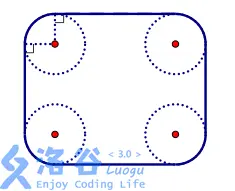
\includegraphics[width=0.5\textwidth]{../Images/Vector3.png}
    \end{figure}

    \textbf{輸入說明}

    輸入的第一行是一個正整數 $n$,表示信用卡的張數。第二行包含三個實數 $a, b, r$,分別表示信用卡(圓滑處理前)豎直方向的長度、水平方向的長度,以及 $\frac{1}{4}$ 圓的半徑。

    之後 $n$ 行,每行包含三個實數 $x, y, \theta$,分別表示一張信用卡中心(即對角線交點)的橫、縱坐標,以及繞中心逆時針旋轉的弧度。
    
    \textbf{輸出說明}

    輸出只有一行,包含一個實數,表示凸包的周長,四捨五入精確到小數點後2位。

    \textbf{範例測試}

    \begin{tabular}{|m{7cm}|m{7cm}|}
        \hline
        範例輸入 1 & 範例輸出 1 \\
        \hline
        \verb|2| & \verb|21.66| \\
        \verb|6.0 2.0 0.0| & \\
        \verb|0.0 0.0 0.0| & \\
        \verb|2.0 -2.0 1.5707963268| & \\
        \hline
    \end{tabular}

    